\documentclass[a4paper,12pt]{article}
% Package to make citations superscrit with brackets
\usepackage[super,square]{natbib}
% Package to change margin size
\usepackage{anysize}
\marginsize{2cm}{2cm}{1cm}{2cm}
% Package to make headers
\usepackage{fancyhdr}
\renewcommand{\headrulewidth}{0pt}
% Package for highligths
\usepackage{soul}
% Colors for the references links
\usepackage[dvipsnames]{xcolor}
% Package to link references
\usepackage{hyperref}
\usepackage{graphicx}
\usepackage{float}
\usepackage{amsmath}
\usepackage{revsymb}

\usepackage{amsfonts}
\usepackage[italian]{babel}
\hypersetup{
    colorlinks=true,
    linkcolor=black,
    citecolor=CadetBlue,
    filecolor=CadetBlue,      
    urlcolor=CadetBlue,
}
% Package for lorem ipsum
\usepackage{lipsum}
% Package for multicolumn
\usepackage{multicol}

\usepackage{xparse}
\usepackage{physics}

\usepackage{multicol,caption}
% Package for removing paragraph identations
\usepackage{parskip}
\setlength\columnsep{18pt} 
\setlocalecaption{italian}{figure}{Fig.}
\setlocalecaption{italian}{table}{Tab.}
\counterwithin{figure}{section} % comandi per numerazione interna di figure, tabelle ed equazioni
\counterwithin{table}{section}
\counterwithin{equation}{section}

 
\begin{document}
\begin{center}
\Large{\textbf{Appunti di Introduzione alla Fisica Nucleare e Subnucleare}}
\vspace{0.4cm}
\normalsize
\\ \textbf{Università degli Studi di Torino a.a. 2025-2026}\\Prof. Riccardo Bellan, appunti di Paolo Rocchietti March\footnote{paolo.rocchiettimarc@edu.unito.it} \\

\vspace{0.1cm}
%\textit{Organization}
\medskip
\normalsize
\end{center}
\vspace{0.4cm}
{\color{gray}\hrule}
\medskip
\begin{figure}[H]
    \centering
    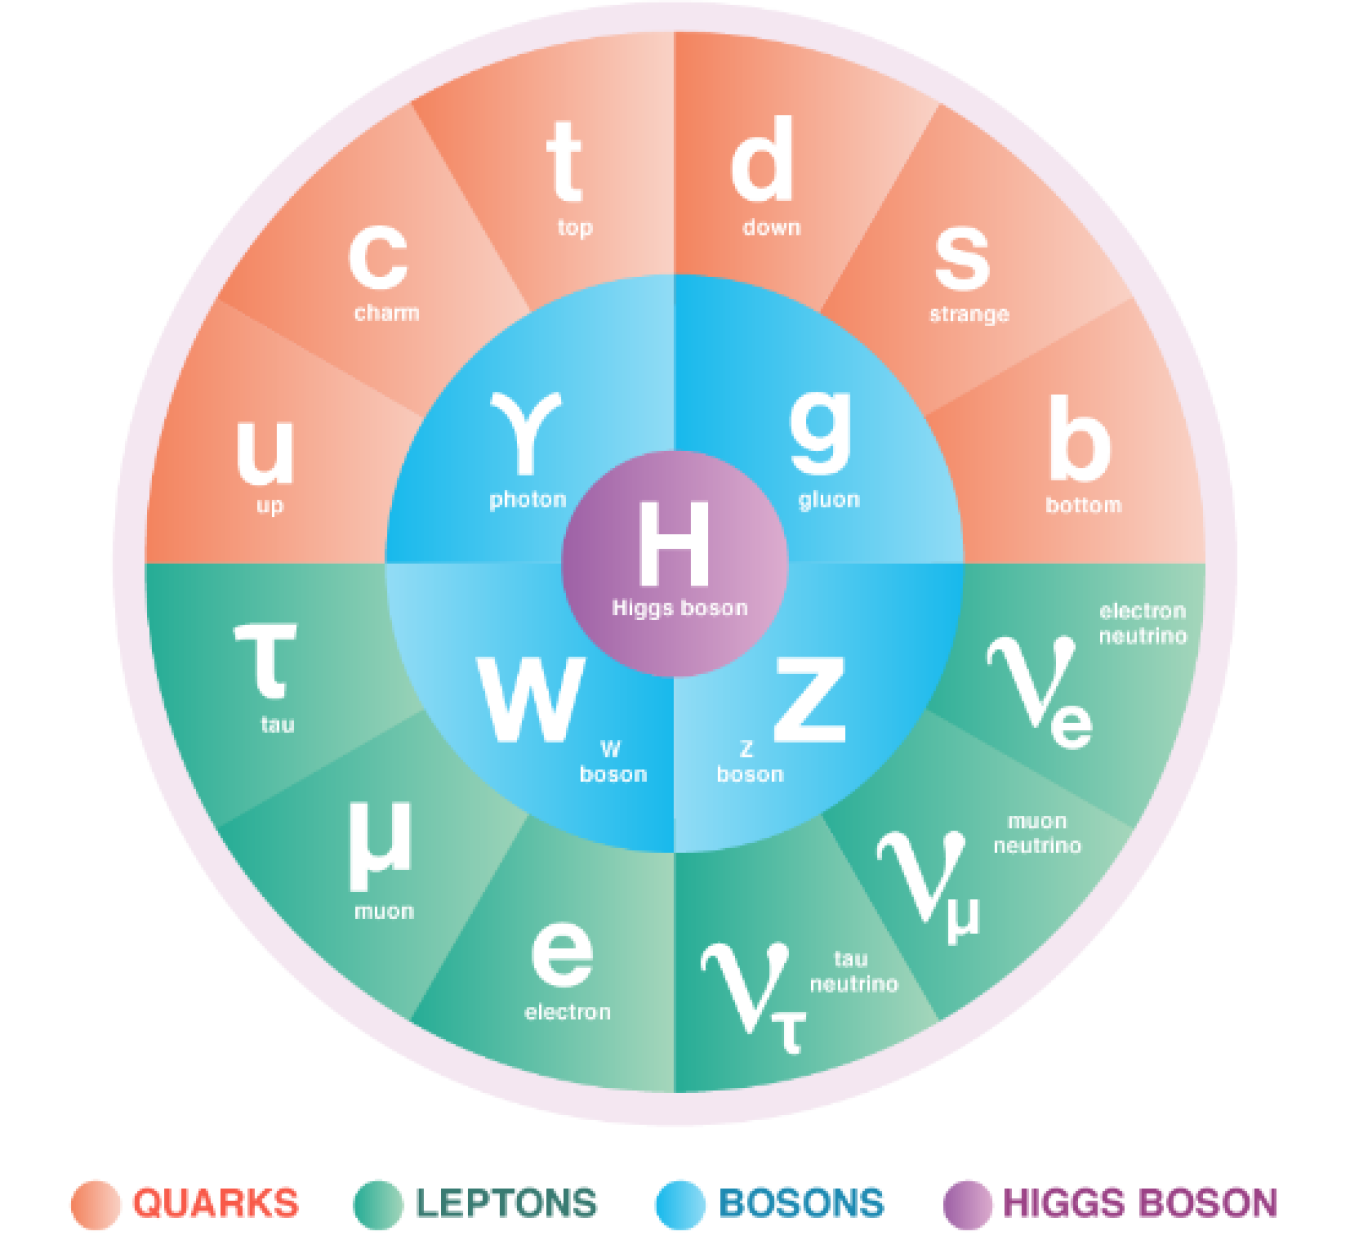
\includegraphics[width = 0.9\linewidth]{std_model.png}
\end{figure}
\newpage
Questi sono i miei appunti del corso di IFNS, tenuto per il canale B del corso di 
laurea in Fisica dell'Università di Torino dal prof. Riccardo Bellan nell'a.a.
2025-2026. 


Non ne garantisco la totale correttezza, ma spero che possano essere d'aiuto.

\tableofcontents
%lezione del 26 febbraio 2026
\section{Introduzione e ripasso}
\subsection{Unità di misura e costanti fisiche}
Nell'ambito della fisica nucleare e subnucleare, come in ogni altro della fisica,
esistono delle unità di misura non appartenenti al SI che però risultano più
utilizzate per praticità:
\begin{itemize}
    \item Lunghezza: $1 fm = 10^{-15}m$, femtométro o Fermi;
    \item Energia: scala da $1 GeV$ a $ 1 TeV $, con $ 1GeV = 1.602 \cdot 10^{-10} J$;
    \item Massa: si usano i $ GeV/c^2 $, da $E=mc^2$;
    \item Momento (impulso): $ GeV/c $; 
\end{itemize}

È anche importante ricordare qualche costante fisica:
\begin{itemize}
    \item Velocità della luce nel vuoto: $ c = 2.997 \cdot10^8 m/s $;
    \item $\hbar c = 197.3 MeV\cdot fm$;
    \item Massa del protone: $M_p = 938.272 MeV/c^2$;
    \item Massa del neutrone: $M_n = 939.565 MeV/c^2$;
    \item Massa dell'elettrone: $m_e = 510.998 MeV/c^2$;
    \item Costante di struttura fine: $\alpha = \frac{e^2}{4\pi \epsilon_0 \hbar c}\approx \frac{1}{137.04}$;
\end{itemize}
\subsection{Ripasso: cinematica relativistica}
Si ricordano qui i concetti fondamentali della cinematica relativistica.

L'usuale spazio delle configurazioni $ \mathbb{R}^3$ viene sostituito dallo spazio
di Minkowski $ M $, uno spazio vettoriale a 4 dimensioni con un prodotto scalare
pseudo-riemanniano rappresentato dalla matrice diag$ (+,-,-,-) $: gli elementi di
$ M $ sono detti \textit{quadrivettori} e, usualmente, la prima componente rappresenta
la parte "temporale" della grandezza considerata, mentre le altre sono il (tri)vettore
classico corrispondente, ad esempio $ x = (ct,\vec{x}) $.

Il prodotto scalare segue la metrica sopra riportata, di modo che, dati
$ a = (a_0,\vec{a})$ e $ b = (b_0,\vec{b}) $,  
$a\cdot b = a_0b_0 - \vec{a}\cdot\vec{b}$: è noto che il risultato di prodotti scalari
tra quadrivettori è invariante per trasformazioni di Lorentz e che quindi è
indipendente dal sistema di riferimento.
 
Si considerino il quadrimpulso $p = (\frac{E}{c},\vec{p})$ e la quadrivelocità
$u = \gamma(c,\vec{v})$ (con $ \gamma = \frac{1}{\sqrt{1-\beta^2}} $ e
$\beta = \frac{v}{c}$); per definizione, $p = mu = \gamma(mc,m\vec{v})$ e dunque
$$ p^2 = p\cdot p = \gamma^2m^2c^2 - \gamma^2m^2v^2 = \gamma^2m^2c^2(1-\beta^2) = m^2c^2 $$
Dall'altra definizione di $p$ si trova dunque
$$ p^2 = \frac{E^2}{c^2} - |\vec{p}|^2 = m^2c^2 \rightarrow E^2 = |\vec{p}|^2c^2 + m^2c^4$$
si tratta della relazione di \textit{mass-shell} che, per $\vec{p} = 0$, si riduce alla nota
espressione dell'energia a riposo $E = mc^2 $.

Ponendo $E = T + mc^2$, si trova la relazione tra il momento e l'energia cinetica
$$ |\vec{p}|c = \sqrt{T^2 + 2mc^2T} $$

\subsection{Rapporti tra relatività e meccanica quantistica}
Si trova una relazione interessante mescolando quanto appena ricavato, il concetto 
di lunghezza d'onda di De Broglie e l'indeterminazione momento-posizione di Heisenberg:

De Broglie: $ |\vec{p}| = \hbar k = \frac{\hbar}{\lambda} \rightarrow \lambda = \frac{\hbar}{|\vec{p}|}$

Heisenberg: $ \Delta x \Delta p \geq \hbar/ 2$, che può essere approssimato a
$ \Delta x \Delta p \geq \hbar$: se si considera un errore piccolo su $|p|$, cioè
$ \frac{\Delta p }{|\vec{p}|} << 1 $, si ha che
$$ |\vec{p}|\Delta x > \hbar \rightarrow \Delta x > \frac{\hbar}{|\vec{p}|} = \frac{\lambda}{2\pi} := \lambdabar$$ 
cioè che il potere risolutivo sulla posizione di una particella è al più uguale alla
sua lunghezza di De Broglie ridotta.

In termini relativistici, $\lambdabar$ è legata all'energia cinetica $T$:

$$\lambdabar = \frac{\hbar c}{|\vec{p}|c} = \frac{\hbar c}{\sqrt{T^2 + 2mc^2T}}$$

Al CERN, per esempio, per protoni $m_p = 1 GeV/c^2$ con energia $ T = 13TeV $, si ha
un massimo possibile di risoluzione spaziale $\lambdabar \approx 1.5 \cdot 10^{-5} fm$.

\subsection{Equazione di Klein-Gordon}

Si consideri ora l'equazione di Schrödinger libera
$$ i \hbar\pdv{\psi}{t}=\frac{-\hbar^2}{2m}\laplacian\psi \rightarrow \hat{E}\psi = \hat{H}\psi$$
definendo gli operatori $ \hat{E} = i \hbar \pdv{t} $ e $ \hat{H} = \frac{\hat{p}^2}{2m} $.

Questa relazione ha senso solo in un contesto non relativistico per alcune ragioni:
\begin{itemize}
    \item Il tempo $ t $ è un parametro, mentre $ \vec{x}$ è un operatore, mentre nella meccanica
	relativistica sono trattati come due variabili spaziali;
    \item L'equazione è di primo ordine in $ t $, mentre di second'ordine in $ \vec{x} $;
    \item L'osservabile $ \bra{\psi} \dv{\vec{x}}{t}\ket{\psi} $ (valor medio della velocità) non è
	limitato a $ c $, come prevede la relatività speciale. 
\end{itemize}

Per questi motivi, bisogna trovare un'altra formulazione per unire le due teorie:
un metodo è prendere la relazione di mass-shell e promuoverne i termini a operatori

$$ E^2 = |\vec{p}|^2c^2 + m^2c^4, \quad \hat{E}=i \hbar\pdv{t},\quad \hat{p}^2 = -\hbar^2\laplacian$$
$$-\hbar^2 \pdv[2]{\psi}{t} = -\hbar^2c^2\laplacian\psi + m^2c^4\psi$$ 

Questo risultato è \textbf{l'equazione di Klein Gordon}, scritta anche in forma covariante come
$$ (\hbar^2\partial^{\mu}\partial_{\mu} + m^2c^2)\psi = 0 $$ 

Una soluzione di questa equazione è, come atteso, una funzione d'onda del tipo
$$ \psi(x) = exp\{-\frac{i}{\hbar}p\cdot x\} $$
dove $ x $ e $ p $ sono quadrivettori.

In questo contesto, risulta fisicamente accettabile considerare $ E<0 $, infatti 
$$ \pdv{\psi}{t} = p_0c\psi = \pm\sqrt{|\vec{p}|^2c^2+m^2c^4}\psi$$
Al segno negativo si può dare il significato di particelle con energia positiva,
ma che viaggiano nello spazio-tempo in direzione negativa: diventerà evidente dall'equazione di Dirac
che queste sono \textit{antiparticelle}. [TO BE CONTINUED...]

%lezione del 04/03/2026
%tenuta dal prof costa del corso A: non capisco come unire le lezioni in un discorso
%coerente e sensato: per ora le butto insieme e vedrò
\newpage
NOTE TO SELF: qui iniziano le lezioni di Costa (04/03), non c'è un filo che lega a prima,
da rivedere per cercare di darci un senso, probabilmente farà K-G dopo.
\section{Teoria degli urti}
Nella fisica nucleare e subnucleare, gli urti giocano un ruolo fondamentale:
a differenza della meccanica classica, descrivono dei processi in maniera molto
precisa (quando due biglie collidono non sono davvero puntiformi, quando lo fanno due
elettroni sì): per trattarli si userà la cinematica relativistica.

Si adotta da ora in poi, se non specificato, la notazione per cui il quadrimomento di una
particella $ a $  viene denotato con lo stesso nome della particella:
$ a = (\frac{E_a}{c},\vec{a}) $.

Si consideri ora l'urto tra due particelle $ a $ e $ b $; esse possono urtare in due modi: 
\begin{itemize}
    \item Urto elastico: le particelle rimangono le medesime, ma i loro quadrimomenti cambiano;	
    \item Urto anelastico: le particelle possono cambiare a seguito dell'interazione.
\end{itemize}
In entrambi i casi il quadrimomento totale è conservato:
$$ a + b = a' + b',\quad a + b = e + f + g $$ 
nel caso, rispettivamente, di urto elastico e non elastico.

Si noti che la quantità $ a^2 = \frac{E_a^2}{c^2} - |\vec{a}| = m_a^2c^2$ è un invariante,
quindi è una caratteristica della particella, detta \textbf{massa invariante}.

\subsection{Cinematica degli urti elastici}
Si considera ora il semplice caso di una particella $ a $ che urta contro un target, costituito
da particelle $ b $: la conservazione del quadrimomento è
$$ a + b = a' + b' $$
Vale anche la conservazione dei moduli quadri
$$ (a+b)^2 = (a'+b')^2 \rightarrow a^2 + b^2 +2a\cdot b =a'^2 + b'^2 +2a'\cdot b' $$
poiché $ a $ e $ a' $ sono la stessa particella, la loro massa invariante è uguale:

$a^2 = a'^2$, similmente $b^2 = b'^2$.

%\bibliographystyle{plain}
%\bibliography{references}
\end{document}
